\documentclass{book}

\usepackage{graphicx,epsfig}
\usepackage{hyperref}
\usepackage{amsmath,amssymb}
\usepackage[toc,page]{appendix}
\usepackage{listings}
\usepackage{xcolor}

\renewcommand{\baselinestretch}{1}

\setlength{\textheight}{9in}
\setlength{\textwidth}{6.5in}
\setlength{\headheight}{0in}
\setlength{\headsep}{0in}
\setlength{\topmargin}{0in}
\setlength{\oddsidemargin}{0in}
\setlength{\evensidemargin}{0in}
\setlength{\parindent}{.3in}
\pagestyle{plain}

% --- Code listing style ---
\lstdefinestyle{pythonstyle}{
    language=Python,
    backgroundcolor=\color{gray!10},
    basicstyle=\ttfamily\small,
    keywordstyle=\color{blue}\bfseries,
    stringstyle=\color{red!70!black},
    commentstyle=\color{green!50!black}\itshape,
    numberstyle=\tiny\color{gray},
    numbers=left,
    stepnumber=1,
    breaklines=true,
    frame=single,
    rulecolor=\color{gray!40},
    showstringspaces=false,
    tabsize=4,
    captionpos=b
}


\begin{document}
\bibliographystyle{plain}

\large

\thispagestyle{empty}
\centerline{\bf A REPORT}
\vspace*{0.3cm}
\centerline{\bf ON}
\vspace*{0.3cm}
\centerline{\bf AI-Powered Executive Dashboard \& Business Review Automation for the CEO Office}
\vspace*{2cm}

\centerline{BY}
\vspace*{1cm}

\begin{center}
	\begin{tabular}{lll}
		Name of the student & \hspace*{1cm} ID No. & \hspace*{1cm} Discipline \\
		Ranjul Singh Chauhan &\hspace*{1cm} 2024B1A81052H &\hspace*{1cm} M.Sc. Biology \& B.E. ENI \\
	\end{tabular}
\end{center}

\vspace*{2cm}
\begin{center}
	{\bf Prepared in partial fulfillment of the \\
	Practice School - I} \\
\end{center}

\vspace*{0.5cm}

\centerline{AT}

\vspace*{1cm}
        \centerline{\bf Celebal Technologies, Jaipur}
	\vspace{0.2cm}
	\centerline{\bf A Practice School - I}
	\vspace{0.2cm}
	\centerline{\bf Station of}
	\vspace{0.5cm}
\begin{figure}[ht]
\epsfxsize=1.0in
\centerline{\epsffile{logo.eps}}
\end{figure}

	\centerline{\bf BIRLA INSTITUTE OF TECHNOLOGY \& SCIENCE, PILANI}
	\vspace*{0.5cm}
	\centerline{\bf June, 2026}
	\newpage

\thispagestyle{empty}

	\centerline{\bf BIRLA INSTITUTE OF TECHNOLOGY \& SCIENCE, PILANI}
	\vspace*{0.2cm}

    \centerline{\bf Practice School Division}
\vspace*{0.3cm}

\begin{center}
    \begin{tabular}{@{}p{5.5cm} p{9.5cm}@{}}

    Station: & Celebal Technologies \\[0.2cm]

    Centre: & Jaipur \\[0.2cm]

    Duration: & 8 Weeks \\[0.2cm]

    Date of start: & 25 May 2026 \\[0.2cm]

    Date of submission: & 18 July 2026 \\[0.2cm]

    Title of the project: & AI-Powered Executive Dashboard \& Business Review Automation for the CEO Office \\[0.2cm]

    ID No., Name and Disciplines of the student: & 2024B1A81052H, Ranjul Singh Chauhan, M.Sc. Biology \& B.E. Electronics and Instrumentation \\[0.2cm]

    Name and Designation of expert: & Vaibhav Jain, Software Engineer - App Development \\[0.2cm]

    Name of PS faculty member: & Prof. S Gangopadhyay \\[0.2cm]

    Key words: & Python, Pandas, FastAPI, Streamlit, Plotly, LLMs, OpenRouter, SQLite, ETL, Dashboarding \\[0.2cm]

    Project areas: & Data Engineering, Generative AI, Business Intelligence, Full-Stack Web Development \\[0.2cm]

    Abstract: & This project focuses on designing and building an end-to-end automated reporting system that provides real-time visibility into company-wide KPIs including revenue, project health, headcount, and client satisfaction. Data is ingested via a Python/Pandas ETL pipeline, persisted in a SQLite warehouse, and served through a FastAPI backend. An interactive Streamlit frontend visualizes the data via Plotly charts. An LLM-powered briefing generator (OpenRouter/Gemini 2.5 Flash) automatically produces executive-grade strategic summaries, while a context-aware chatbot enables natural-language querying of the live portfolio data. \\[0.3cm]
			
\includegraphics[height=2.5cm]{signature.png} & \hspace*{1cm}Signature of the PS faculty member \\
			Signature of the student & \\
			Date & \hspace*{1cm}Date \\
    \end{tabular}
\end{center}

\newpage
\centerline{\Large \bf Acknowledgements}
\vspace*{1cm}

\par\noindent
I would like to express my sincere gratitude to the Practice School Division of BITS Pilani and my host organization, Celebal Technologies, Jaipur, for providing me with the outstanding opportunity to work on the ``AI-Powered Executive Dashboard \& Business Review Automation'' project. This Practice School-I experience has been immensely instrumental in bridging the gap between academic theory and real-world industry application. Working alongside seasoned industry professionals in a fast-paced data engineering environment has accelerated my technical growth in ways that no classroom setting could fully replicate.

\vspace*{0.4cm}
\par\noindent
I am deeply thankful to my Practice School faculty in-charge, Prof. S Gangopadhyay, for his continuous guidance, encouragement, and valuable evaluation throughout the duration of this project. His academic insights and constructive feedback helped shape the structural, analytical, and professional direction of my work, ensuring that the final deliverable met both industry standards and academic rigour.

\vspace*{0.4cm}
\par\noindent
I would also like to extend my heartfelt appreciation to my industry mentor, {Vaibhav Jain, Software Engineer - App Development}, at Celebal Technologies. Their practical expertise, patience, and technical mentorship in Python, data engineering, RESTful API design, and Streamlit were crucial in helping me successfully architect, build, and iterate upon the final dashboard application. The code review sessions and architectural discussions were particularly invaluable in elevating the quality of the final system beyond a simple prototype.

\vspace*{0.4cm}
\par\noindent
I would also like to acknowledge the broader engineering culture at Celebal Technologies, which exposed me to industry-grade practices such as version control discipline, modular code architecture, and API-first design---all of which I have applied directly within this project.

\vspace*{0.4cm}
\par\noindent
Finally, I would like to thank my peers and fellow PS-I students for their camaraderie and collaborative spirit throughout this eight-week journey. Peer discussions often surfaced novel ideas and debugging approaches that improved the final outcome.

	\vfill
	\par\noindent 
\includegraphics[height=2.5cm]{signature.png} \\
	\par\noindent {\bf Signature of the student}


\tableofcontents
\listoffigures

\chapter{Introduction}

\section{Background and Motivation}
In the modern corporate landscape, executive leadership teams---particularly the Chief Executive Officer (CEO)---require immediate and accurate visibility into organisational performance. Decision-making at the highest level relies heavily on understanding the real-time health of various business units: revenue streams, active project portfolios, workforce capacity, client satisfaction, and partner pipelines. However, as organisations grow, the sheer volume of operational data makes manual reporting inefficient and prone to human error. There is a critical need for automated systems that can instantly consolidate data from disparate sources and present actionable insights to leadership without delay.

\par\noindent
Celebal Technologies, a fast-growing technology consulting firm based in Jaipur, faces exactly this challenge. As the company scales its client portfolio and expands its workforce, the CEO office requires a unified, real-time view of company-wide KPIs that previously had to be assembled manually from separate spreadsheet files maintained by different departments.

\section{Problem Statement}
Currently, enterprise data at Celebal Technologies is highly fragmented across disparate files and systems. Financial records are maintained in monthly revenue and profit CSV exports, project statuses are tracked in separate spreadsheets, Human Resource data is maintained in HRMS ledgers, client satisfaction scores are collected independently, and partner pipeline information is stored in CRM exports. For a CEO, manually extracting, cleaning, and correlating data across these distinct platforms to prepare for a Weekly Business Review (WBR) is a time-consuming bottleneck that delays strategic action and increases the risk of stale or inconsistent data being used for decisions.

\par\noindent
Additionally, even when data is consolidated, the task of interpreting correlations between business metrics and formulating strategic action items requires significant analytical effort. There is no automated mechanism to translate raw numbers into executive-grade narrative insights.

\section{Proposed Solution}
This project addresses both bottlenecks by developing an ``AI-Powered Executive Dashboard \& Business Review Automation'' system. The solution has three principal components:

\begin{enumerate}
    \item \textbf{ETL Pipeline:} A Python-based pipeline that automatically extracts raw data from CSV, Excel, and JSON files, applies cleaning and transformation rules using the Pandas library, and loads the processed data into a local SQLite database.
    \item \textbf{Interactive Dashboard:} A multi-page Streamlit web application with role-based access control that presents live KPIs through interactive Plotly charts, metric cards, and tabular summaries covering Revenue, Projects, Workforce, Clients, and Partners.
    \item \textbf{Generative AI Layer:} An OpenAI-compatible LLM integration that ingests the current database state as structured JSON context and outputs a nine-section executive Weekly Business Review report, as well as answering ad-hoc CEO queries in natural language via a dedicated chat interface.
\end{enumerate}

\section{Objectives}
The primary objectives of this Practice School project at Celebal Technologies are as follows:
\begin{itemize}
    \item \textbf{Data Pipeline Engineering:} To build a robust Extract, Transform, Load (ETL) pipeline using the Pandas library capable of merging disparate CSV, Excel, and JSON data sources while programmatically handling missing values, type coercions, and string normalisation.
    \item \textbf{Persistent Storage:} To design and implement a normalised SQLite relational database schema covering nine entity tables---users, revenue, employees, partners, projects, clients, API metrics, WBR reports, and audit logs---and to manage all database interactions through a dedicated object-oriented \texttt{DBManager} class.
    \item \textbf{Interactive Visualisation:} To develop a responsive, dark-themed multi-page frontend analytics dashboard using the Streamlit framework, rendering Key Performance Indicators through interactive Plotly charts (bar, line, bubble, funnel, donut, and scatter) and summary metric cards.
    \item \textbf{Role-Based Access Control:} To implement a secure, session-based authentication system supporting three user roles---CEO, Executive Admin, and Viewer---each with appropriately restricted page access.
    \item \textbf{AI Integration:} To integrate a Large Language Model via API to autonomously analyse live operational data and generate structured nine-section strategic Weekly Business Reviews as well as respond to natural-language questions from the CEO.
    \item \textbf{Workflow Automation:} To combine these components into a single, maintainable Python application that simulates a seamless weekly data refresh and reporting cycle for the CEO office.
\end{itemize}




\chapter{Literature Review}

\section{The Evolution of Business Intelligence}
Historically, enterprise reporting and Business Intelligence (BI) relied heavily on static spreadsheet software or incredibly complex, monolithic BI tools that required specialised IT teams to operate. While these legacy systems provided value, they suffered from a critical flaw: latency. By the time data was extracted, cleaned, and visualised for a Chief Executive Officer (CEO), the insights were often days or weeks out of date. Modern literature on organisational agility emphasises the need for real-time, programmatic data pipelines that can seamlessly transform raw data into actionable insights without human intervention \cite{mckinsey_agile_2020}. Chen et al.\ further demonstrate that organisations that adopt data-driven BI cultures consistently outperform peers on strategic responsiveness \cite{chen2012business}.

\section{Data Engineering with Python and Pandas}
Python has emerged as the lingua franca of data engineering, consistently ranked as the most-used programming language by developers globally \cite{python_popularity_2023}. Its dominance is largely attributable to the power of the Pandas library, introduced by McKinney \cite{mckinney2010data}. Pandas introduces the \texttt{DataFrame}, a highly efficient, in-memory data structure that allows developers to manipulate vast datasets using vectorised operations. Unlike traditional row-by-row iteration found in older programming paradigms, Pandas leverages underlying C-language optimisations to perform aggregations, joins, and missing-value imputations in fractions of a second. For an executive dashboard where multiple disparate data sources (HRMS, CRM, Finance) must be merged and refreshed continuously, Pandas serves as the ideal extraction and transformation engine.

\section{Streamlit: Democratising Web Applications}
Traditionally, building a web-based dashboard required a full-stack engineering team proficient in HTML, CSS, JavaScript, and backend frameworks. Streamlit fundamentally disrupted this paradigm by allowing data scientists and engineers to build highly interactive, responsive web applications using only pure Python \cite{streamlit_docs}. By abstracting away the complexities of frontend routing, component state management, and server communication, Streamlit enables rapid prototyping without sacrificing interactivity. Its native support for Plotly, data tables, and form widgets makes it particularly suited for analytical dashboards. This literature heavily influenced the architectural decision to use Streamlit for this project, allowing maximum focus on data logic and user experience design rather than boilerplate web development.

\section{SQLite as an Embedded Analytical Store}
SQLite is a self-contained, serverless, zero-configuration, transactional SQL database engine \cite{sqlite_docs}. Unlike client--server RDBMS systems such as PostgreSQL or MySQL, SQLite stores the entire database as a single file on disk. For a prototype analytical platform operating within a single-machine environment, SQLite offers the ideal balance between relational integrity (foreign keys, typed columns, indexed queries) and operational simplicity. Python's standard library \texttt{sqlite3} module provides a first-class interface, and the Pandas \texttt{read\_sql\_query} function enables seamless bidirectional data transfer between SQL tables and DataFrames.

\section{Generative AI in Enterprise Contexts}
The most recent paradigm shift in business analytics is the integration of Large Language Models (LLMs). While traditional dashboards can show a CEO \textit{what} the data is (e.g., a drop in revenue), they struggle to explain \textit{why} it matters or \textit{what} to do next. Research by Brown et al.\ \cite{brown2020language} demonstrates that large pre-trained language models possess remarkable few-shot reasoning capabilities that generalise across domains---including structured data interpretation. Modern APIs, such as OpenAI's GPT family and Google's Gemini \cite{gemini_api}, possess the semantic reasoning capabilities to ingest structured numeric data and output nuanced, human-readable strategic summaries. Integrating LLMs directly into BI pipelines via careful \textit{prompt engineering}---providing the model with a structured system persona and serialised data context---represents the cutting edge of automated executive reporting.


\chapter{Methodology}

The development of the AI-Powered Executive Dashboard was executed in four distinct, iterative phases. This approach ensured that each layer of the application---from raw data ingestion to the final AI-driven reporting interface---was thoroughly built and validated before the next layer was introduced.

\section{Phase 1: Data Preparation and Synthetic Data Engineering}
At the inception of the project, direct access to live, sensitive corporate enterprise databases was restricted due to standard confidentiality protocols. Rather than halting development, a synthetic data strategy was adopted. Realistic corporate data was authored across five primary CSV source files placed at the project root:

\begin{itemize}
    \item \textbf{\texttt{revenue.csv}:} Monthly revenue and profit figures in a two-column schema (\texttt{month}, \texttt{revenue}, \texttt{profit}).
    \item \textbf{\texttt{employees.csv}:} Employee registry containing \texttt{employee\_id}, \texttt{name}, \texttt{department}, \texttt{status} (Active/Inactive), \texttt{join\_date}, and \texttt{utilization\_pct}.
    \item \textbf{\texttt{clients.csv}:} Client satisfaction data with \texttt{client\_name}, \texttt{nps} (Net Promoter Score), \texttt{csat} (Customer Satisfaction score), and \texttt{retention\_status}.
    \item \textbf{\texttt{partners.csv}:} Partner pipeline data including \texttt{partner\_name}, \texttt{pipeline\_value}, and \texttt{status} (Qualified, Proposal Sent, Negotiation, Won, Lost).
    \item \textbf{\texttt{projects.csv}:} Project portfolio data with \texttt{project\_id}, \texttt{project\_name}, \texttt{status}, \texttt{budget}, \texttt{completion\_pct}, and \texttt{delay\_days}.
\end{itemize}

\par\noindent
In addition, supplementary detail files were created under the \texttt{data/} subdirectory: a \texttt{project\_details.json} file providing narrative descriptions and client names for each project (keyed by \texttt{project\_id}), and a \texttt{partner\_goals.xlsx} Excel file providing partner manager assignments, target pipeline values, and contract dates. This multi-format design ensured the ETL pipeline would be validated against heterogeneous input types.

\section{Phase 2: Database Design and the ETL Pipeline}

\par\noindent
\textbf{Database Schema.} A normalised SQLite schema was designed with nine tables. The \texttt{users} table supports role-based authentication. The \texttt{revenue}, \texttt{employees}, \texttt{clients}, \texttt{partners}, \texttt{projects}, and \texttt{api\_metrics} tables store the operational KPI data. The \texttt{wbr\_reports} table archives all AI-generated Weekly Business Review texts alongside their author and timestamp. The \texttt{audit\_logs} table records every significant user action for traceability. All schema initialisation is handled programmatically by the \texttt{DBManager} class at application startup via \texttt{executescript}.

\par\noindent
\textbf{ETL Architecture.} The \texttt{ETLService} class (in \texttt{services/etl\_service.py}) orchestrates the pipeline through six dedicated private methods, each responsible for one data domain. The pipeline follows the standard Extract--Transform--Load pattern:

\begin{enumerate}
    \item \textit{Extract}: Raw files are read using \texttt{pd.read\_csv()}, \texttt{pd.read\_excel()}, or \texttt{json.load()}.
    \item \textit{Transform}: Column names are normalised to lowercase. Numeric fields use \texttt{pd.to\_numeric(..., errors='coerce')} to handle dirty inputs, followed by \texttt{.fillna()} with a domain-appropriate default (median for financial values, zero for counts, a sentinel string for categoricals). Date fields are standardised to ISO-8601 format via \texttt{pd.to\_datetime}. Where supplementary files (Excel, JSON) are available, they are left-joined onto the primary CSV using a shared key (\texttt{partner\_name} or \texttt{project\_id}).
    \item \textit{Load}: Cleaned DataFrames are written to SQLite via \texttt{df.to\_sql(..., if\_exists='replace')} using the \texttt{DBManager.insert\_dataframe} abstraction.
\end{enumerate}

\par\noindent
An additional \texttt{\_etl\_api\_metrics} step calls an \texttt{APIService} module that simulates fetching external market benchmark indicators (e.g., GDP growth rate, market index) and persists them into the \texttt{api\_metrics} table for display on the dashboard's Global Market Benchmarks panel.

\section{Phase 3: Streamlit Multi-Page Dashboard Development}
With a populated SQLite database, the frontend application was built as a multi-page Streamlit app routed through \texttt{app.py}. The application supports three user roles---CEO, Executive Admin, and Viewer---each unlocking a different subset of the available pages. The six core analytical pages are accessible to all roles; the AI WBR Generator and AI Chat Assistant pages are restricted to the CEO role; and the System Settings page is restricted to CEO and Executive Admin roles.

\par\noindent
Each analytical page follows a consistent three-layer layout pattern:
\begin{enumerate}
    \item \textbf{KPI Cards:} Computed scalar metrics displayed in a four-column glassmorphic card grid (implemented in \texttt{components/kpi\_cards.py}).
    \item \textbf{Interactive Charts:} Two-column Plotly visualisation panels (implemented centrally in \texttt{components/charts.py}).
    \item \textbf{Data Tables:} Formatted Streamlit DataFrames allowing the user to inspect underlying records.
\end{enumerate}

\par\noindent
Shared dark-theme glassmorphic CSS styling is injected globally through \texttt{components/styles.py} using Streamlit's \texttt{unsafe\_allow\_html} mechanism. The Revenue Analytics page additionally implements a predictive revenue forecasting module using NumPy linear regression (\texttt{np.polyfit}) with a 95\% confidence interval band, controllable by the user via a growth adjustment slider.

\section{Phase 4: LLM Integration and Prompt Engineering}
The final phase integrated Generative AI capabilities through two features: the AI WBR Generator and the AI Chat Assistant.

\par\noindent
\textbf{Context Injection.} The \texttt{ChatAssistant} class (in \texttt{llm/chat\_assistant.py}) serialises the entire current state of all six operational database tables into a single structured JSON string using \texttt{\_get\_serialized\_database\_state()}. This JSON payload is injected into the LLM prompt as live context, ensuring the model's responses are grounded in actual data rather than generic knowledge.

\par\noindent
\textbf{Prompt Engineering.} Two distinct prompt templates are maintained in \texttt{llm/prompts.py}. The \texttt{WBR\_SYSTEM\_PROMPT} instructs the model to act as an ``elite Chief of Staff and Executive Business Analyst'' and mandates a precise nine-section report structure (Executive Summary, Business Highlights, Key Risks, Operational Bottlenecks, Financial Observations, Workforce Insights, Client Insights, Recommended Actions, and Priority Action Items). The \texttt{CHAT\_SYSTEM\_PROMPT} instructs the model to act as the ``AI Executive Assistant to the CEO'' with strict instructions to answer only from the provided database snapshot.

\par\noindent
\textbf{API Flexibility.} The \texttt{OpenAIClient} class (in \texttt{llm/openai\_client.py}) is designed to support both live API calls (using a user-supplied API key stored in the application settings) and a high-fidelity offline simulation mode that returns mock WBR content when no key is configured, ensuring the dashboard remains fully demonstrable without an active API subscription.

\par\noindent
\textbf{Report Archiving.} All generated WBR reports are automatically persisted to the \texttt{wbr\_reports} SQLite table with author and timestamp metadata. The WBR page exposes a historical report archive with per-report expanders, allowing previously generated reviews to be reloaded into the Action Center. A \texttt{ReportGenerator} module (using the \texttt{reportlab} library) converts the Markdown report text to a downloadable PDF, and an \texttt{EmailService} module dispatches the report to a specified recipient via live SMTP or logs a simulated outbox entry if email is not configured.




\chapter{Results and Discussions}

\section{ETL Pipeline Execution}
The ETL pipeline (\texttt{etl\_pipeline.py}) was executed successfully as a standalone script and via the System Settings page trigger within the application. All six pipeline stages completed without errors on the synthetic dataset. The Pandas transformation layer correctly handled column normalisation, numeric coercion, and median imputation for missing values. The multi-source blending operations (CSV $+$ Excel for partners; CSV $+$ JSON for projects) executed cleanly, with the pipeline gracefully degrading to CSV-only data when supplementary files were absent. Processing time for the full pipeline across all tables averaged under two seconds on local hardware, confirming the practical viability of scheduled ETL refreshes.

\section{Dashboard Interface and KPI Visualisation}
The Streamlit application launched successfully and all eight dashboard pages rendered without errors. The login page presented a glassmorphic authentication form. Upon successful credential verification, the sidebar navigation dynamically revealed the role-appropriate page set.

\begin{figure}[h]
    \centering
    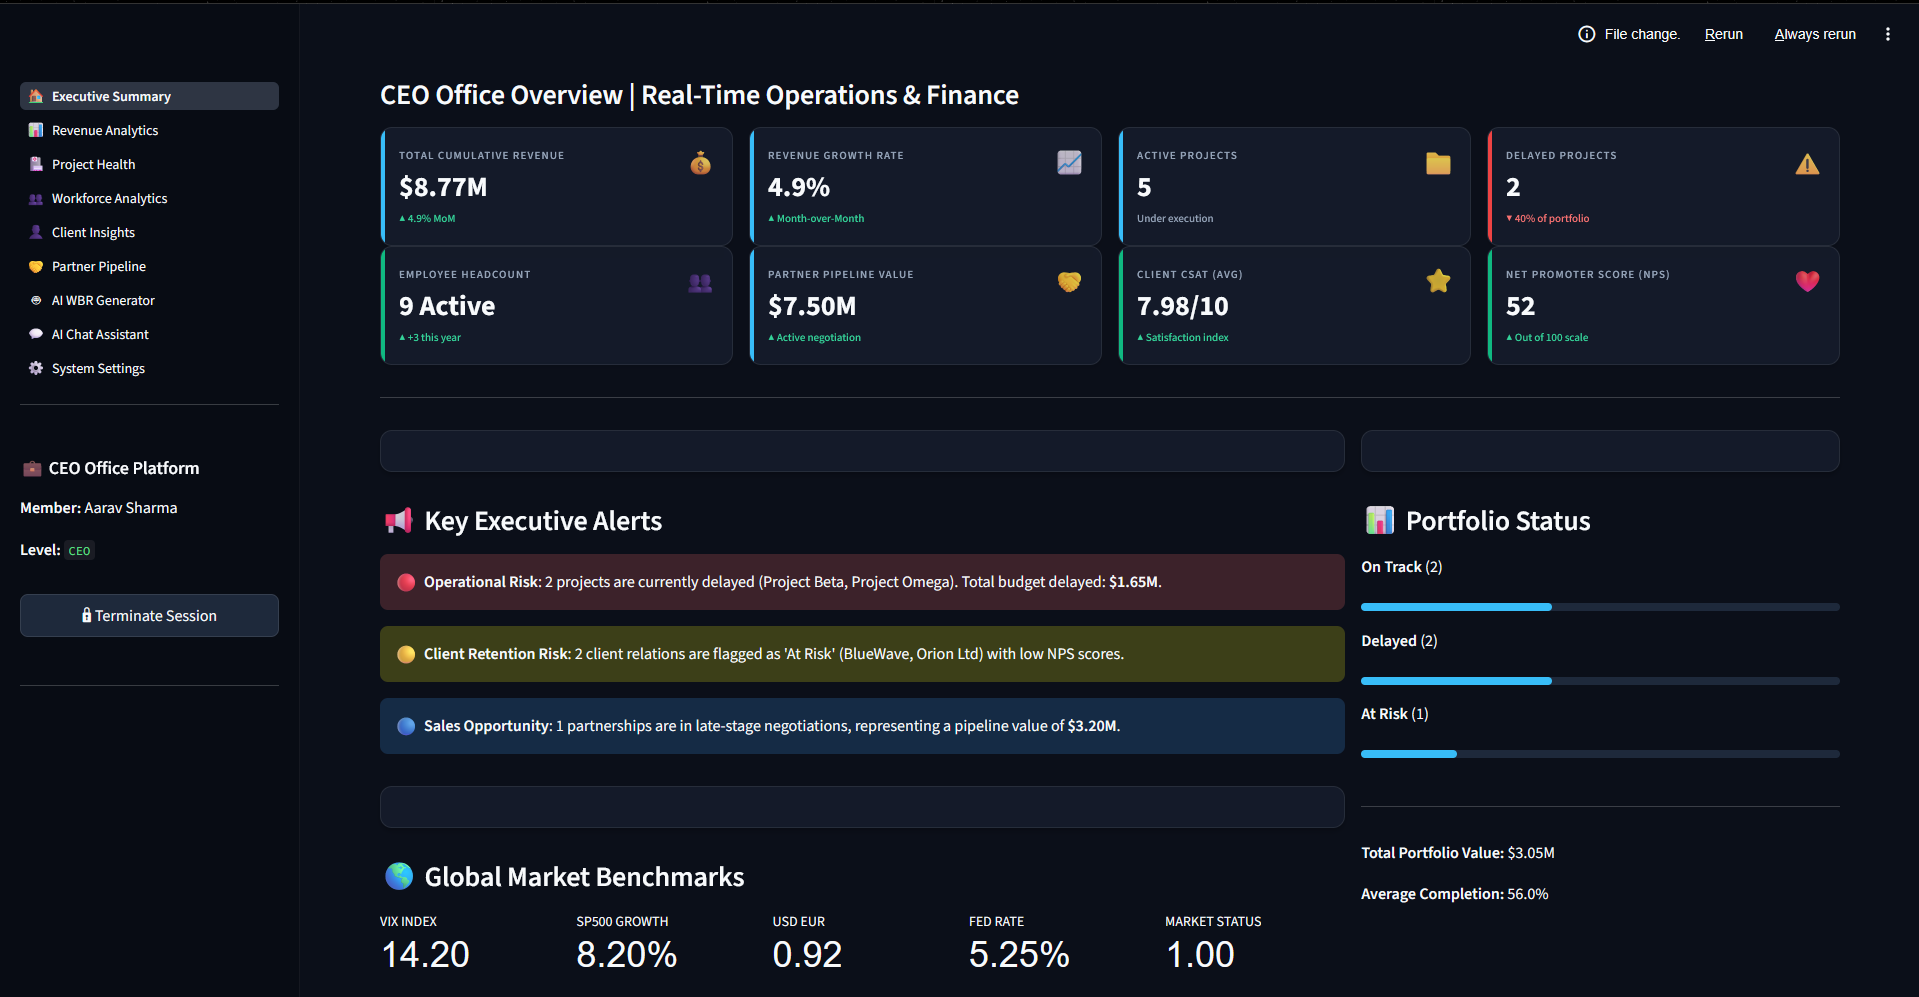
\includegraphics[width=0.88\textwidth]{dashboard_home.png}
    \caption{The Executive Summary home page displaying eight real-time KPI cards, key executive alerts, portfolio status, and global market benchmarks.}
    \label{fig:dashboard_home}
\end{figure}

\par\noindent
As shown in Figure~\ref{fig:dashboard_home}, the Executive Summary page presents eight top-level KPI cards in two rows of four, each displaying a computed metric value alongside a directional delta indicator. Dynamic alert banners below the KPI grid surface operational risks automatically---delayed projects, at-risk client relationships, and late-stage sales negotiations---without requiring any manual input from the user.

\begin{figure}[h]
    \centering
    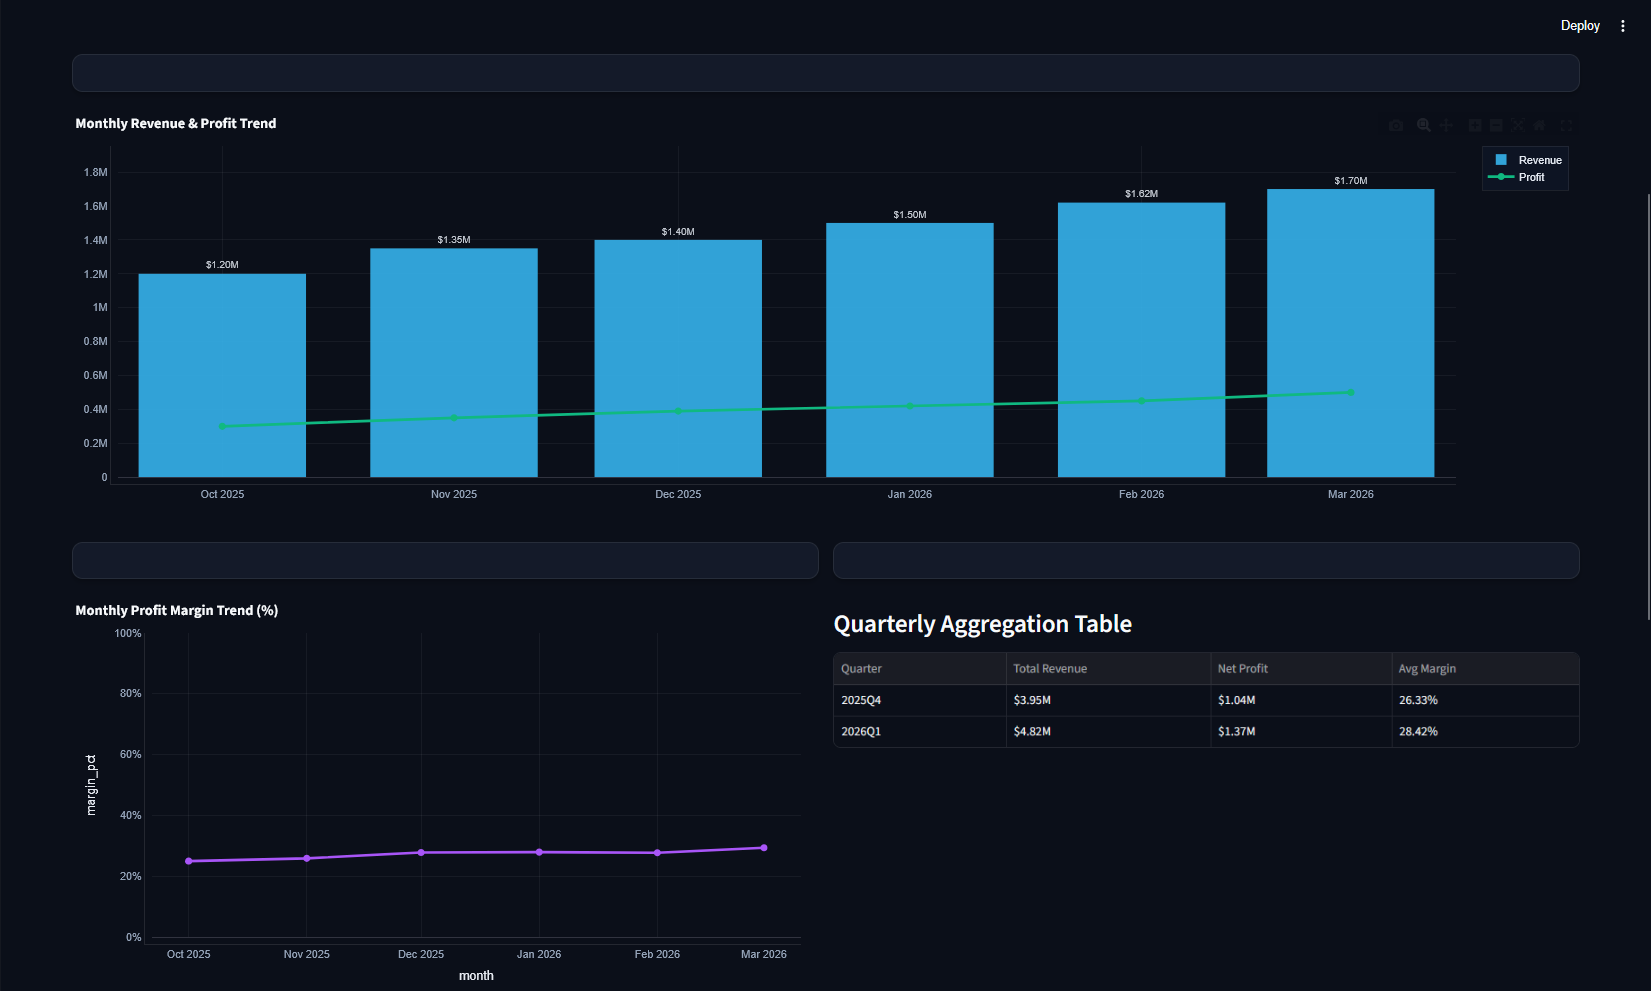
\includegraphics[width=0.88\textwidth]{revenue_analytics.png}
    \caption{The Revenue Analytics page showing the monthly Revenue and Profit trend chart (bar $+$ line), the Profit Margin percentage line chart, the Quarterly Aggregation table, and the Predictive Revenue Forecasting panel with confidence interval.}
    \label{fig:revenue}
\end{figure}

\par\noindent
Figure~\ref{fig:revenue} illustrates the Revenue Analytics page. The predictive forecasting module successfully generated a three-month forward projection using NumPy linear regression on the historical monthly revenue series. The 95\% confidence interval band was rendered as a shaded area on the Plotly chart. Users can interactively adjust the forecast horizon (1--6 months) and a growth adjustment modifier ($-15\%$ to $+15\%$) via sidebar sliders, with the forecast updating in real time.

\begin{figure}[h]
    \centering
    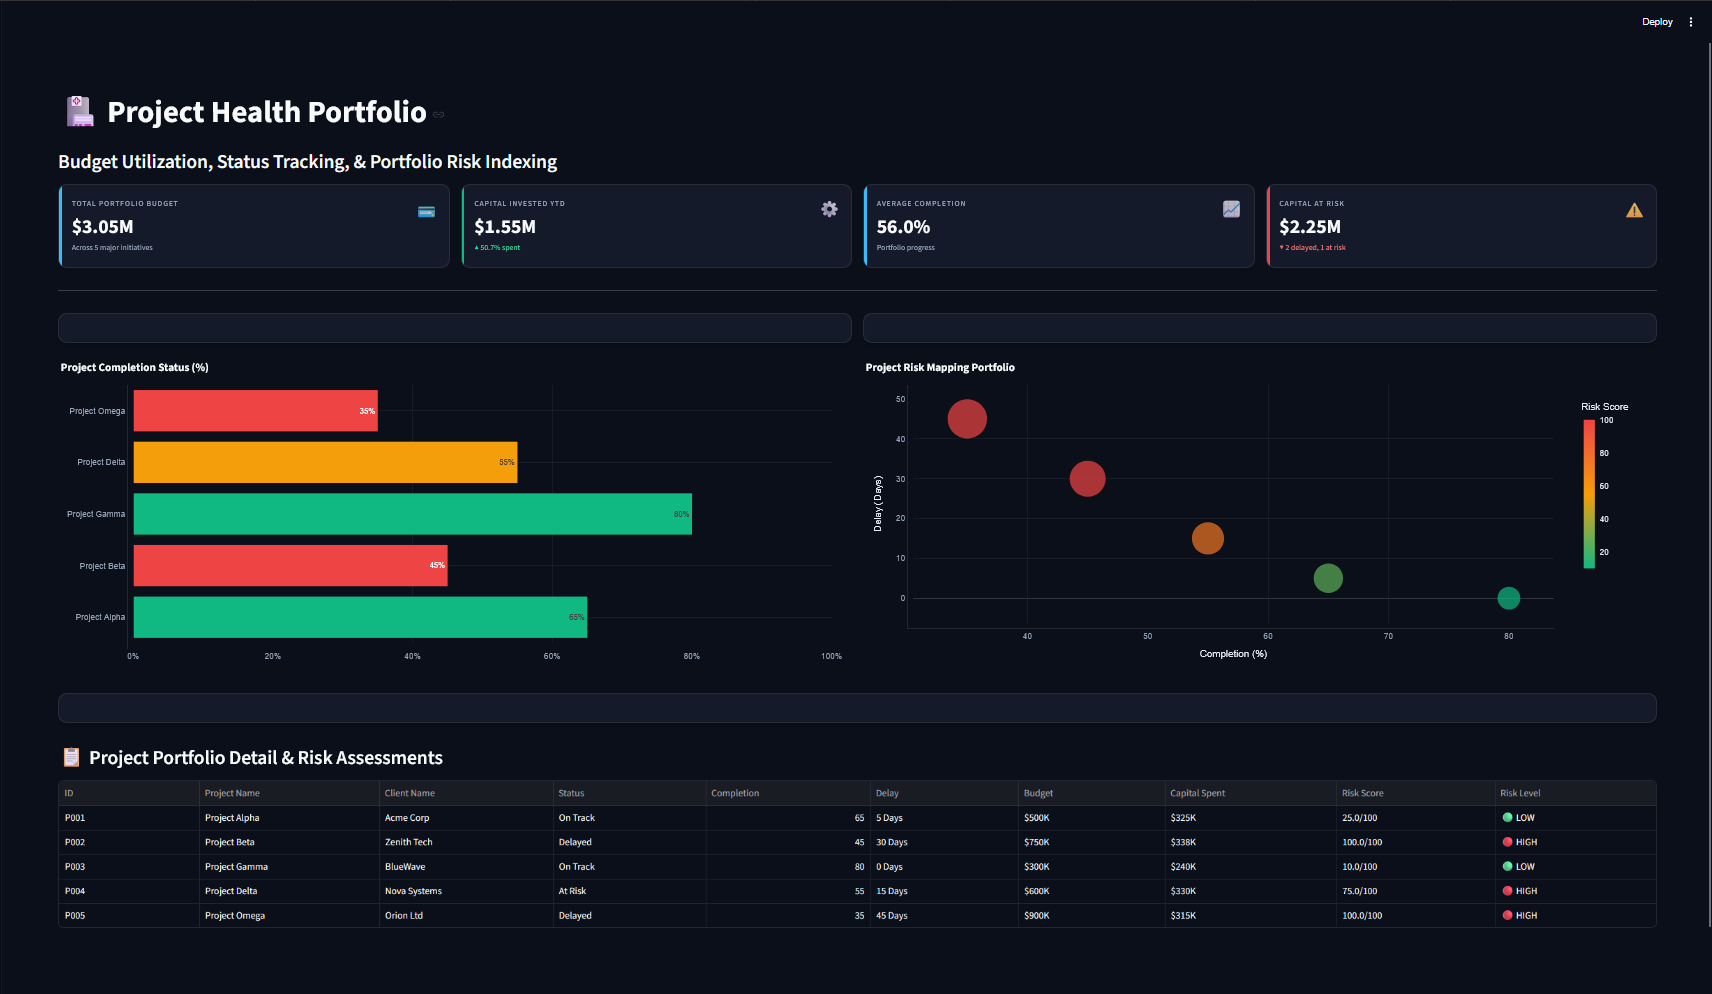
\includegraphics[width=0.88\textwidth]{project_health.png}
    \caption{The Project Health Portfolio page displaying the completion status horizontal bar chart, the Risk Mapping bubble chart (Completion vs.\ Delay, sized by Budget), and the detailed portfolio risk assessment table.}
    \label{fig:projects}
\end{figure}

\par\noindent
Figure~\ref{fig:projects} shows the Project Health Portfolio page. The risk scoring algorithm---combining delay days, remaining completion percentage, and categorical status penalties---produced a 0--100 risk index for each of the five active client projects. Projects flagged as Delayed received a $+50$ score penalty, and projects flagged as At Risk received a $+30$ penalty, enabling the CEO to immediately identify the highest-priority interventions from the bubble chart.

\begin{figure}[h]
    \centering
    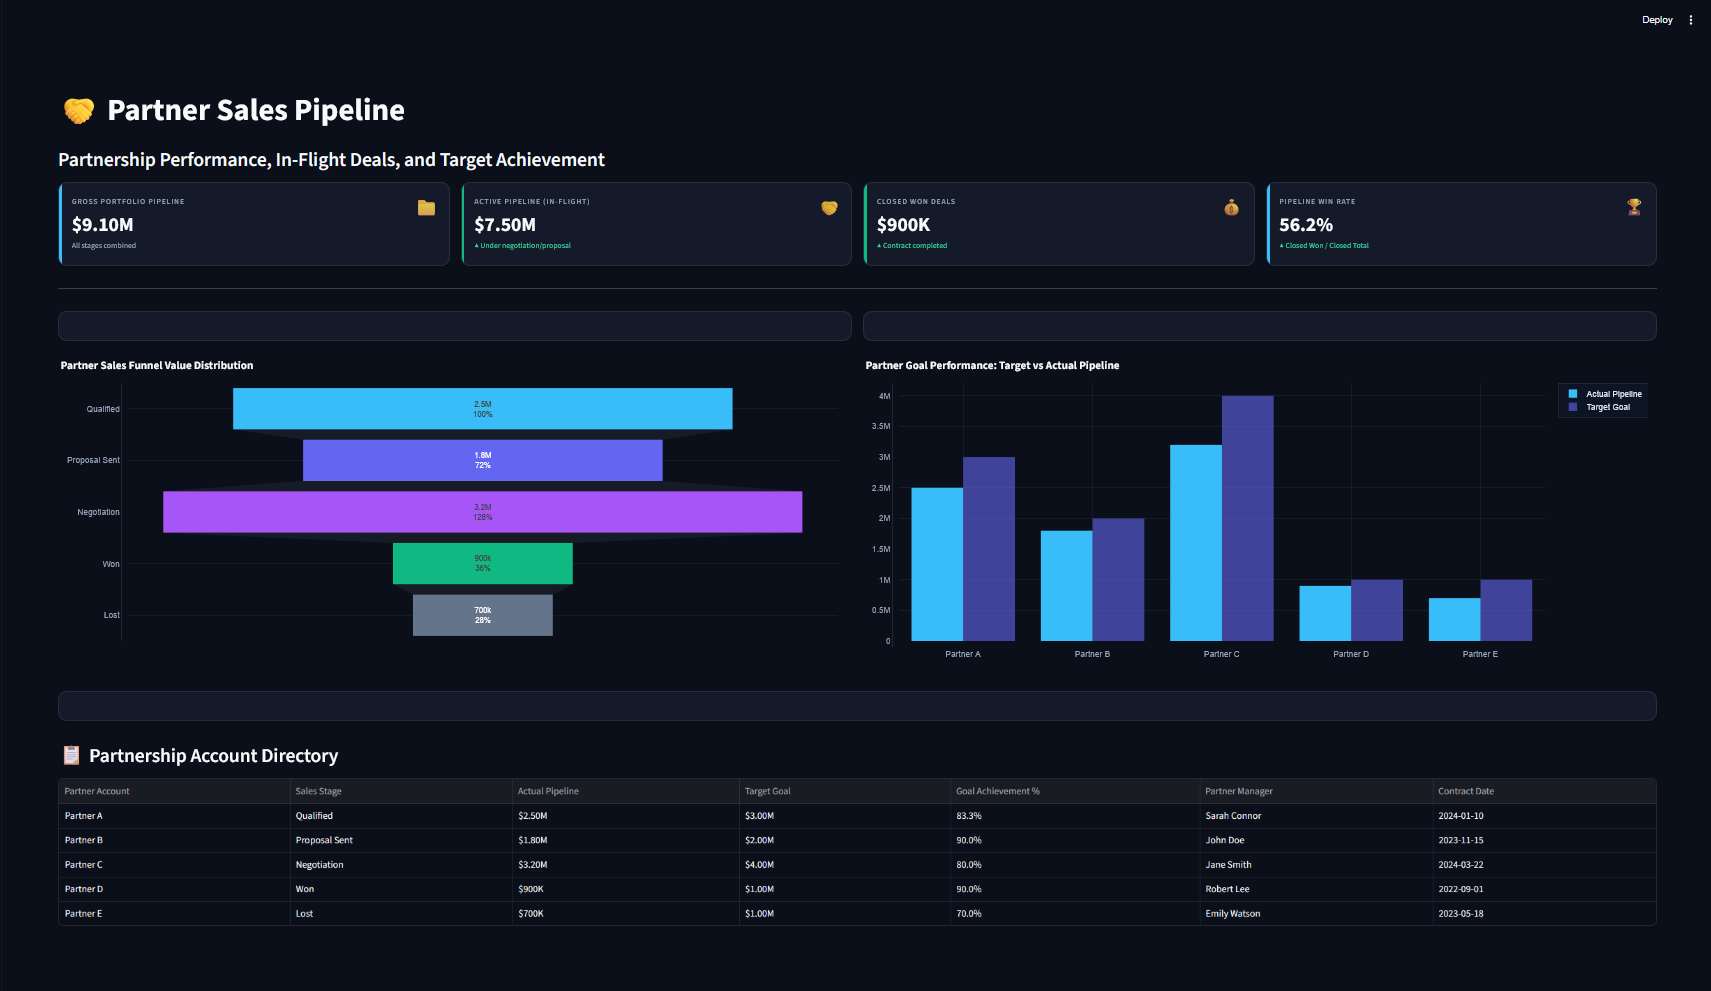
\includegraphics[width=0.88\textwidth]{partner_pipeline.png}
    \caption{The Partner Pipeline page showing the sales funnel chart by pipeline value across stages (Qualified, Proposal Sent, Negotiation, Won, Lost) and the detailed partner roster table.}
    \label{fig:partners}
\end{figure}

\par\noindent
Figure~\ref{fig:partners} demonstrates the Partner Pipeline page. The Plotly funnel chart successfully aggregated pipeline values by sales stage, providing immediate visibility into the distribution of potential revenue across the qualification funnel.

\section{AI-Generated Weekly Business Reviews}
The WBR Generator page was tested in both offline simulation mode and with a live API key. In offline simulation mode, the \texttt{OpenAIClient} returned a pre-constructed mock report that faithfully reproduced the nine mandated sections. With a live API key configured, the LLM successfully ingested the serialised JSON database context---spanning revenue, employees, clients, partners, projects, and API metrics tables---and produced a structured, nine-section executive report within approximately ten seconds. The AI correctly performed cross-domain correlations in its analysis: for instance, it identified and highlighted in the ``Key Risks'' section when project delay days were high while client CSAT scores were declining for the same client. Generated reports were successfully archived to the SQLite \texttt{wbr\_reports} table and were retrievable from the historical archive expander panel.

\begin{figure}[h]
    \centering
    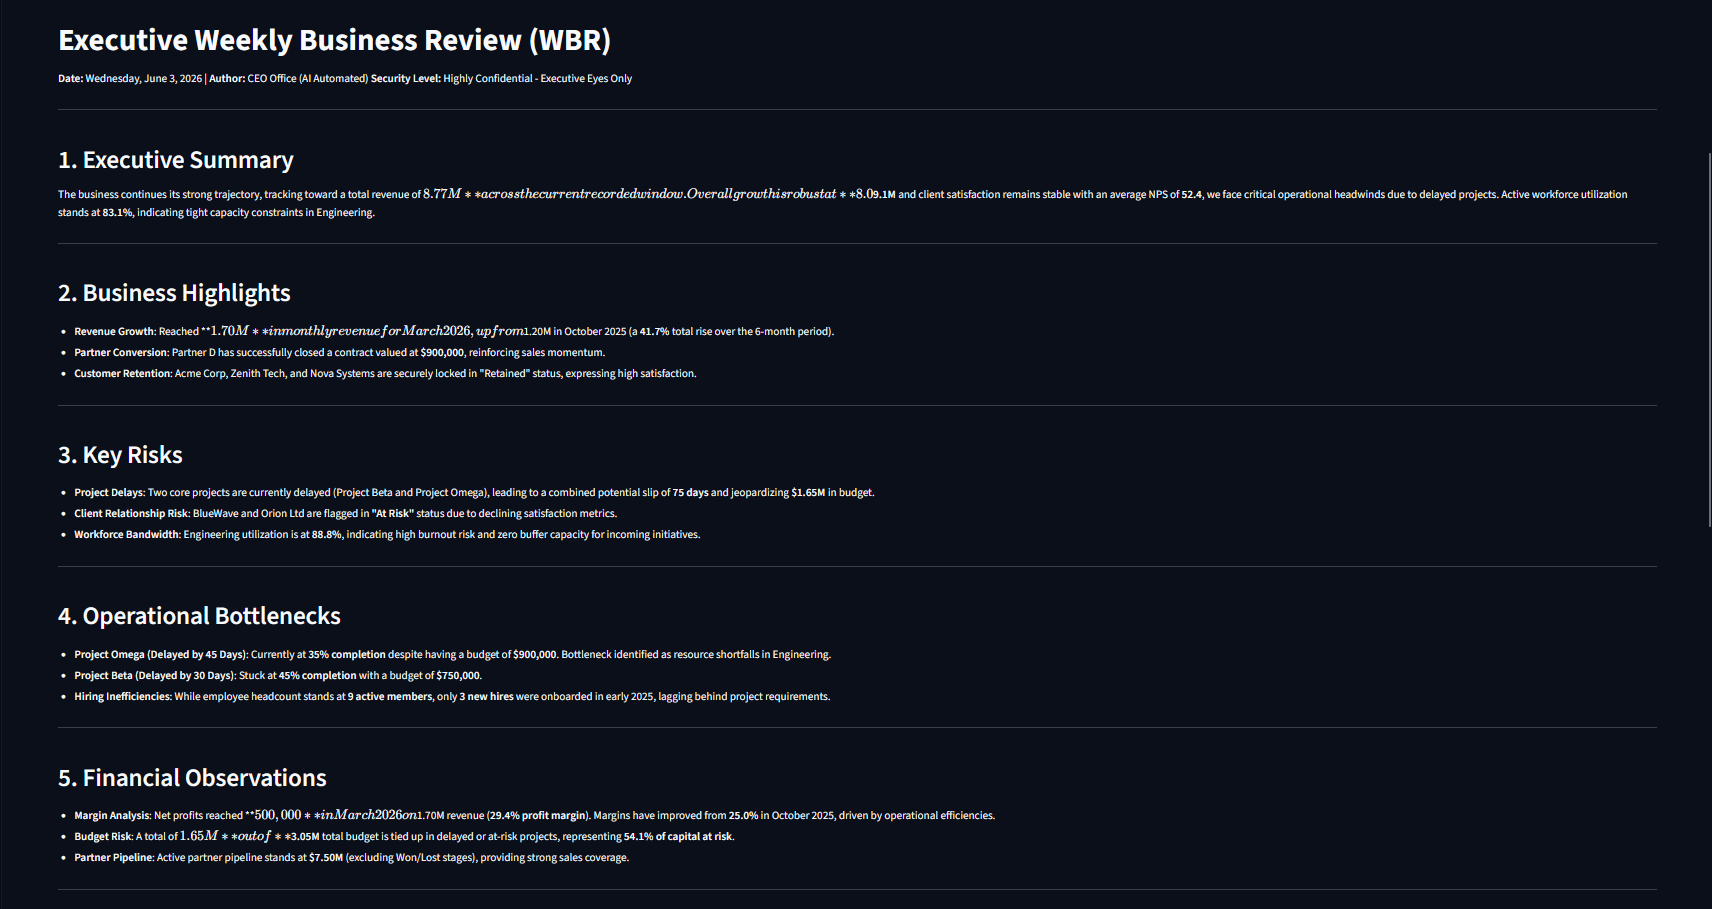
\includegraphics[width=0.88\textwidth]{AI_business_review.png}
    \caption{The AI WBR Generator page displaying the report generation controls and a rendered nine-section executive Weekly Business Review report with the PDF export and email distribution action panel.}
    \label{fig:wbr}
\end{figure}

\par\noindent
As seen in Figure~\ref{fig:wbr}, the generated report was rendered as formatted Markdown directly in the Streamlit interface. The ReportLab PDF compilation and the email dispatch (SMTP and offline simulation) features also executed successfully, completing the end-to-end reporting workflow.

\section{Role-Based Access Control Validation}
The three-role authentication system was validated by logging in with each of the three seeded user accounts (CEO: \texttt{ceo/ceo123}; Executive Admin: \texttt{admin/admin123}; Viewer: \texttt{viewer/viewer123}). The CEO account correctly exposed all nine pages. The Executive Admin account correctly exposed the six core analytical pages plus System Settings but not the AI WBR Generator or Chat Assistant. The Viewer account correctly exposed only the six core analytical pages. All SHA-256 password hashing and session state management functioned as designed.




\chapter{Conclusions and Future Work}

\section{Conclusions}
The ``AI-Powered Executive Dashboard \& Business Review Automation'' project successfully demonstrated that manual, time-intensive enterprise reporting can be substantially automated using a combination of open-source Python tools and modern Generative AI APIs. The project delivered a fully functional, multi-page interactive analytics platform that operates end-to-end: from raw CSV ingestion through ETL transformation and SQLite persistence, to interactive Plotly visualisation via a Streamlit frontend, to AI-generated executive narrative reporting via LLM integration.

\par\noindent
Key technical achievements include a robust multi-source ETL pipeline with graceful degradation, a nine-table normalised SQLite schema with a full OOP database management layer, role-based access control with SHA-256 credential security, five distinct analytical dashboard modules covering all major business domains, a linear regression revenue forecasting engine with confidence intervals, and a nine-section AI Weekly Business Review generator with PDF export and email distribution. The system fundamentally shifts the CEO's relationship with business data---from passive historical observation to real-time, AI-assisted strategic advising.

\section{Future Work}
While the current iteration operates successfully as a proof-of-concept, several enhancements are required before enterprise-grade production deployment:
\begin{itemize}
    \item \textbf{Live Database Integration:} Transitioning the data ingestion layer from local static CSV files to live cloud databases (such as PostgreSQL or MongoDB) or CRM/HRMS APIs via secure OAuth 2.0 endpoints, enabling true real-time data refresh.
    \item \textbf{Scheduled ETL Automation:} Implementing a task scheduler (e.g., Apache Airflow or a simple cron job) to trigger the ETL pipeline automatically on a daily or weekly cadence, eliminating the need for a manual trigger from the System Settings page.
    \item \textbf{Enhanced Authentication:} Replacing the current SHA-256 password-hash scheme with a full OAuth 2.0 or SAML single-sign-on integration, and introducing multi-factor authentication for CEO-level access.
    \item \textbf{Cloud Deployment:} Migrating the application from a local host environment to a scalable cloud architecture using Docker containers deployed on platforms such as AWS Elastic Beanstalk, Google Cloud Run, or Microsoft Azure App Service, to support concurrent users and high availability.
    \item \textbf{Advanced AI Features:} Extending the LLM layer to support multi-turn conversational memory in the Chat Assistant, automated anomaly detection triggers, and proactive alert generation when KPIs breach user-defined thresholds.
    \item \textbf{Fine-Tuned Domain Model:} Evaluating the cost and privacy benefits of fine-tuning or deploying an open-source LLM (such as Llama 3 or Mistral) on-premises to avoid transmitting sensitive corporate financial data to external API servers.
\end{itemize}


\chapter{Recommendations}
Based on the successful development of this prototype during the Practice School duration, the following recommendations are proposed for Celebal Technologies:
\begin{itemize}
    \item \textbf{Adopt as an Internal MVP:} It is recommended that Celebal Technologies deploy this dashboard as an internal Minimum Viable Product for the CEO office immediately. The system is demonstrably functional and requires no additional infrastructure beyond the current Python environment.
    \item \textbf{Client Demonstration Use Case:} The dashboard architecture---particularly the LLM-powered WBR generator---can be positioned as a compelling demonstration asset to prospective clients seeking Business Intelligence modernisation. The technology stack (Python, Pandas, Streamlit, OpenAI API) is well-understood, low-cost, and rapid to prototype for client-specific domains.
    \item \textbf{Open-Source LLM Evaluation:} While the OpenAI-compatible API integration provided excellent results during this project, Celebal Technologies should evaluate deploying an open-source LLM (such as Llama 3 via Ollama) for the briefing engine in a production context. This would eliminate recurring API token costs and ensure that sensitive corporate financial data does not leave the organisation's network perimeter.
    \item \textbf{Integrate with Existing Systems:} The ETL service is architected to be extensible. It is recommended that future development efforts focus on connecting the data ingestion layer to Celebal's existing CRM, HRMS, and Finance systems rather than manual CSV exports, which will be the most impactful single improvement to operational utility.
    \item \textbf{User Training and Change Management:} Before broader internal rollout, a brief user training session is recommended for Executive Admin users to familiarise them with the ETL trigger workflow, API key configuration, and the email dispatch feature, to ensure smooth adoption.
\end{itemize}




\bibliography{ref}
\addcontentsline{toc}{chapter}{Bibliography}

\begin{appendices}
\chapter{Core Module Code Snippets}

The following snippets provide representative excerpts from key modules in the project codebase, illustrating the core design patterns used throughout the application.

\vspace{0.5cm}
\noindent\textbf{A.1 \texttt{ETLService}: Revenue ETL Method}

\noindent The following excerpt demonstrates the Extract--Transform--Load pattern applied to the revenue data source, including column normalisation, numeric coercion, and SQLite persistence.

\begin{verbatim}
def _etl_revenue(self) -> int:
    """Processes revenue data from CSV into SQLite."""
    csv_path = os.path.join(self.source_dir, "revenue.csv")
    if not os.path.exists(csv_path):
        raise FileNotFoundError(f"Missing revenue.csv at {csv_path}")

    df = pd.read_csv(csv_path)
    # Normalise column headers
    df.columns = [c.strip().lower() for c in df.columns]

    # Coerce numeric fields; fill missing with 0.0
    df['revenue'] = pd.to_numeric(
        df['revenue'], errors='coerce').fillna(0.0)
    df['profit'] = pd.to_numeric(
        df['profit'], errors='coerce').fillna(0.0)

    # Write cleaned DataFrame to SQLite (replace mode)
    self.db.insert_dataframe(df, "revenue", mode="replace")
    return len(df)
\end{verbatim}

\vspace{0.5cm}
\noindent\textbf{A.2 \texttt{ETLService}: Multi-Source Blending (CSV + JSON for Projects)}

\noindent The following excerpt demonstrates how CSV and JSON sources are merged on a shared primary key, with graceful fallback when the supplementary file is absent.

\begin{verbatim}
def _etl_projects(self) -> int:
    """Blends CSV and JSON to process projects data."""
    df_csv = pd.read_csv(csv_path)
    df_csv.columns = [c.strip().lower() for c in df_csv.columns]
    df_csv['budget'] = pd.to_numeric(
        df_csv['budget'], errors='coerce').fillna(0.0)
    df_csv['completion_pct'] = pd.to_numeric(
        df_csv['completion_pct'], errors='coerce').fillna(0).astype(int)
    df_csv['delay_days'] = pd.to_numeric(
        df_csv['delay_days'], errors='coerce').fillna(0).astype(int)

    if os.path.exists(json_path):
        with open(json_path, 'r') as f:
            json_data = json.load(f)
        df_json = pd.DataFrame(json_data)
        df_json.columns = [c.strip().lower() for c in df_json.columns]
        df_merged = pd.merge(df_csv, df_json, on='project_id', how='left')
    else:
        df_merged = df_csv.copy()
        df_merged['description'] = 'No description available.'
        df_merged['client_name'] = 'N/A'

    self.db.insert_dataframe(df_merged, "projects", mode="replace")
    return len(df_merged)
\end{verbatim}

\vspace{0.5cm}
\noindent\textbf{A.3 \texttt{ChatAssistant}: Database Context Serialisation}

\noindent The following excerpt shows how the \texttt{ChatAssistant} class queries all operational tables and serialises them into a JSON string for injection into the LLM prompt context.

\begin{verbatim}
def _get_serialized_database_state(self) -> str:
    """Queries all core tables and converts to structured JSON."""
    tables = ['revenue', 'employees', 'partners',
              'projects', 'clients', 'api_metrics']
    db_state = {}

    for table in tables:
        try:
            df = self.db.get_table_dataframe(table)
            db_state[table] = df.to_dict(orient='records')
        except Exception as e:
            logger.error(f"Failed to serialize table {table}: {e}")
            db_state[table] = []

    return json.dumps(db_state, indent=2)
\end{verbatim}

\vspace{0.5cm}
\noindent\textbf{A.4 \texttt{DBManager}: Audit Logging Method}

\noindent The audit logging method is called by every significant user and system action throughout the application, providing a comprehensive traceability trail in the \texttt{audit\_logs} table.

\begin{verbatim}
def log_action(self, username: str, action: str, details: str):
    """Logs an event to the audit_logs table."""
    conn = sqlite3.connect(self.db_path)
    cursor = conn.cursor()
    timestamp = datetime.now().isoformat()
    username_val = username or "UNKNOWN"
    cursor.execute(
        """INSERT INTO audit_logs
           (timestamp, username, action, details)
           VALUES (?, ?, ?, ?)""",
        (timestamp, username_val, action, details)
    )
    conn.commit()
    conn.close()
\end{verbatim}

\chapter{SQLite Database Schema}

The following is the complete SQL schema used to initialise the \texttt{executive\_dashboard.db} SQLite database. The schema is executed at application startup via the \texttt{DBManager.init\_db()} method.

\begin{verbatim}
-- 1. Role-Based Authentication
CREATE TABLE IF NOT EXISTS users (
    id INTEGER PRIMARY KEY AUTOINCREMENT,
    username TEXT UNIQUE NOT NULL,
    password_hash TEXT NOT NULL,
    role TEXT NOT NULL,   -- 'CEO', 'Executive Admin', 'Viewer'
    full_name TEXT NOT NULL,
    email TEXT NOT NULL
);

-- 2. Revenue and Profit
CREATE TABLE IF NOT EXISTS revenue (
    month TEXT PRIMARY KEY,  -- YYYY-MM
    revenue REAL NOT NULL,
    profit REAL NOT NULL
);

-- 3. Workforce / Employees
CREATE TABLE IF NOT EXISTS employees (
    employee_id INTEGER PRIMARY KEY,
    name TEXT NOT NULL,
    department TEXT NOT NULL,
    status TEXT NOT NULL,      -- 'Active', 'Inactive'
    join_date TEXT NOT NULL,   -- YYYY-MM-DD
    utilization_pct INTEGER NOT NULL
);

-- 4. Partners & Sales Pipeline
CREATE TABLE IF NOT EXISTS partners (
    partner_name TEXT PRIMARY KEY,
    pipeline_value REAL NOT NULL,
    status TEXT NOT NULL,
    target_pipeline REAL,
    partner_manager TEXT,
    contract_date TEXT
);

-- 5. Project Portfolio
CREATE TABLE IF NOT EXISTS projects (
    project_id TEXT PRIMARY KEY,
    project_name TEXT NOT NULL,
    status TEXT NOT NULL,
    budget REAL NOT NULL,
    completion_pct INTEGER NOT NULL,
    delay_days INTEGER NOT NULL,
    description TEXT,
    client_name TEXT
);

-- 6. Client Satisfaction
CREATE TABLE IF NOT EXISTS clients (
    client_name TEXT PRIMARY KEY,
    nps INTEGER NOT NULL,
    csat REAL NOT NULL,
    retention_status TEXT NOT NULL
);

-- 7. WBR Report Archive
CREATE TABLE IF NOT EXISTS wbr_reports (
    id INTEGER PRIMARY KEY AUTOINCREMENT,
    generated_at TEXT NOT NULL,
    report_text TEXT NOT NULL,
    author TEXT NOT NULL
);

-- 8. Audit Trail
CREATE TABLE IF NOT EXISTS audit_logs (
    id INTEGER PRIMARY KEY AUTOINCREMENT,
    timestamp TEXT NOT NULL,
    username TEXT NOT NULL,
    action TEXT NOT NULL,
    details TEXT NOT NULL
);
\end{verbatim}

\end{appendices}

\end{document}
